\chapter{Statistical and Probabilistic Foundations of the Feature Space}
\label{ch:gaussian_space}

The framework proposed in this thesis rests on a single working hypothesis: that the class-conditional feature distributions produced by a frozen visual foundation model are well approximated by multivariate Gaussians, and that the resulting decision surfaces can be described in terms of the geometry of the embedding space they live in. This chapter puts together, in one self-contained treatment, the mathematical and statistical tools used throughout this thesis to build and check that hypothesis. We start with the probabilistic modelling framework itself---Bayesian inference, the Maximum A Posteriori decision rule, and its Mixture-of-Gaussians extension. We then turn directly to the Gaussianity assumption these models depend on, presenting the moment-based diagnostics and the formal hypothesis tests, univariate first and then multivariate, including the Henze--Zirkler statistic and its diagonal adaptation, that are later applied empirically in Chapter~\ref{ch:results}. With that assumption in place, we introduce the inter-class separability metrics---the probabilistic Bhattacharyya distance and the geometric Euclidean distance---used to quantify how classes crowd the embedding space as new tasks arrive. We then explain why estimating a covariance matrix in this setting is difficult in the first place, a difficulty commonly known as the curse of dimensionality, and how it can be addressed through regularization; this naturally leads into the spectral tools---Principal Component Analysis and the associated eigenvalue-decay diagnostics---used to describe the intrinsic dimensionality of the feature space and, in turn, to understand why that regularization is needed.

\section{Foundations of Probabilistic Modeling}
\label{sec:framework:probabilistic}

Representing each class as a Gaussian density only makes sense if there is a solid decision rule behind it that says how to actually use that density to classify a new observation. This section builds that rule from the ground up: starting from Bayes' theorem, we arrive at the Maximum A Posteriori (MAP) criterion, which tells us how to pick the most likely class given the observed features, and then extend it to mixtures of Gaussians for classes whose features are better described by more than one cluster. 
\subsection{Bayes Classification}

At its core, Bayes classification is rooted in \textbf{Bayes' Theorem}, which provides a mathematical framework for updating the probability of a hypothesis based on observed evidence. For a classification task, we seek the posterior probability $p(y=c \mid \vec{x})$—the probability that an observation belongs to class $c$ given its observed feature vector $\vec{x}$.

Bayes' Theorem is defined as:
\begin{equation}
	p(y=c \mid \vec{x}) = \frac{p(\vec{x} \mid y=c) \, p(y=c)}{p(\vec{x})}
\end{equation}
where:
\begin{itemize}
	\item $p(y=c \mid \vec{x})$ is the \textbf{posterior} probability.
	\item $p(\vec{x} \mid y=c)$ is the \textbf{likelihood} of the data given the class.
	\item $p(y=c)$ is the \textbf{prior} probability of the class.
	\item $p(\vec{x})$ is the \textbf{evidence} or marginal likelihood, acting as a normalization constant.
\end{itemize}

The objective of a Bayes classifier is to minimize the Bayes risk; in the simplest case, this corresponds to assigning the observation to the class that maximizes the posterior probability.

\subsection{Likelihood-Based Classification}

Likelihood inference provides a coherent framework for updating the probability of a hypothesis as more evidence or information becomes available. In contrast to frequentist approaches that treat parameters as fixed but unknown constants, the Bayesian paradigm treats parameters as random variables characterized by probability distributions.

The connection between Bayes' Theorem and likelihood-based classification lies in the \textbf{Maximum A Posteriori (MAP)} decision rule. Since the evidence $p(\vec{x})$ is constant across all classes for a given observation, the classification decision depends solely on the product of the likelihood and the prior:
\begin{equation}
	p(y=c \mid \vec{x}) \propto p(\vec{x} \mid y=c) \, p(y=c).
\end{equation}

A generative modeling framework can be adopted and class-conditional Gaussian feature distributions can be assumed:
\begin{equation}
	p(\vec{x} \mid y=c)
	=
	\mathcal{N}(\vec{x} \mid \boldsymbol{\mu}_c, \boldsymbol{\Sigma}_c),
\end{equation}
where $\vec{x} \in \mathbb{R}^d$ represents the feature vector, $\boldsymbol{\mu}_c$ is the class mean vector, and $\boldsymbol{\Sigma}_c \succ 0$ is the covariance matrix.

Classification can be performed via MAP inference by maximizing the log-posterior:
\begin{equation}
	\hat{y}
	=
	\arg\max_{c \in \mathcal{Y}}
	\left[
	\log p(\vec{x} \mid y=c) + \log \pi_c
	\right],
\end{equation}
where $\pi_c = p(y=c)$ denotes the class prior.

Substituting the multivariate Gaussian density into the MAP rule, the decision rule becomes equivalent to:
\begin{equation}
	\hat{y}
	=
	\arg\min_{c}
	\left[
	(\vec{x}-\boldsymbol{\mu}_c)^T
	\boldsymbol{\Sigma}_c^{-1}
	(\vec{x}-\boldsymbol{\mu}_c)
	+
	\log |\boldsymbol{\Sigma}_c|
	-
	2\log \pi_c
	\right].
\end{equation}

\subsubsection{Mixture of Gaussians (MoG)}

A Mixture of Gaussians models a complex probability density as a convex combination of $K$ distinct Gaussian components. This approach is fundamental for clustering and density estimation in multi-modal distributions. Therefore, to capture multimodal feature distributions, the class-conditional model can be extended to a mixture:

\begin{equation}
	p(\vec{x} \mid y=c)
	=
	\sum_{k=1}^{K_c}
	\alpha_{c,k}
	\mathcal{N}(\vec{x} \mid \boldsymbol{\mu}_{c,k}, \boldsymbol{\Sigma}_{c,k}),
\end{equation}
where $\alpha_{c,k} \ge 0$ and $\sum_k \alpha_{c,k} = 1$.

The MAP decision rule becomes
\begin{equation}
	\hat{y}
	=
	\arg\max_c
	\left[
	\log
	\left(
	\sum_{k=1}^{K_c}
	\alpha_{c,k}
	\mathcal{N}(\vec{x} \mid \boldsymbol{\mu}_{c,k}, \boldsymbol{\Sigma}_{c,k})
	\right)
	+
	\log \pi_c
	\right].
\end{equation}

This whole classification framework---from the plain Bayes rule to its Gaussian and mixture-of-Gaussians instantiations---is only as good as the assumption it is built on: that class-conditional features are actually well described by a Gaussian in the first place. The remainder of this chapter puts that assumption to work. Section~\ref{sec:method:gaussianity_main} tests it directly through moment-based diagnostics and formal hypothesis tests; Section~\ref{sec:method:separability} studies how the resulting Gaussians relate to one another as more classes are added; Section~\ref{sec:gsc:covariance} addresses the practical difficulty of estimating a covariance matrix $\boldsymbol{\Sigma}_c$ in a high-dimensional, small-sample regime; and Section~\ref{sec:gsc:spectral} closes the chapter by examining the geometric structure of the space these covariances live in.

\section{Gaussianity Assumptions and Analysis}
\label{sec:method:gaussianity_main}

The validity of the Bayes classifier introduced in Section~\ref{sec:framework:probabilistic} depends on how well the class-conditional Gaussian distributions approximate the true data distribution. The covariance estimators and downstream classification framework proposed in this thesis rest on the working assumption that class-conditional features are approximately Gaussian in the embedding space of visual foundation models (such as DINOv2). The following analytical framework establishes the statistical basis for these assumptions and, subsequently, the concrete methodology used to validate them empirically without relying on manual semantic labels, employing a multi-layered statistical evaluation on the training split of our datasets.

Our validation is structured across two levels, examined in that order in the rest of this section:
\begin{enumerate}
	\item \textbf{Per-Dimension (Univariate) Gaussianity:} Evaluated using moment-based shape diagnostics, the formal D'Agostino--Pearson omnibus normality test, and a coordinate-wise application of the Henze--Zirkler (HZ) test.
	\item \textbf{Per-Class (Multivariate) Gaussianity:} Evaluated in the native high-dimensional feature space using a specialized diagonal-covariance adaptation of the HZ test to circumvent sample-size rank deficiencies.
\end{enumerate}

\subsection{Univariate Gaussianity: Conceptual Diagnostics}
\label{sec:method:gaussianity:univariate_concept}

A first layer of theoretical justification involves examining the univariate properties of individual feature components: the kurtosis and skewness of each coordinate's marginal distribution.

\paragraph{Kurtosis} This statistic measures the ``tailedness'' and peakedness of a probability distribution relative to a normal distribution \cite{joyce2011kurtosis}. As illustrated in Figure \ref{fig:kurtosis}, a perfectly Gaussian distribution has an excess kurtosis of zero (mesokurtic). Distributions with high kurtosis (leptokurtic, $Kurtosis > 0$) exhibit sharper peaks and heavier tails, indicating a higher concentration of data around the mean and a greater likelihood of extreme outliers. Conversely, low kurtosis (platykurtic, $Kurtosis < 0$) indicates a flatter peak and thinner tails.

\begin{figure}[ht]
	\centering
	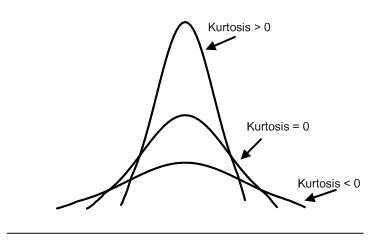
\includegraphics[width=0.37\textwidth]{imagenes/marco/kurtosis.png}
	\caption{Visual representation of kurtosis levels: leptokurtic ($>0$), mesokurtic ($=0$) and platykurtic ($<0$) distributions \cite{joyce2011kurtosis}.}
	\label{fig:kurtosis}
\end{figure}

\paragraph{Skewness} This measure quantifies the asymmetry of a distribution around its mean. As shown in Figure \ref{fig:skewness}, a symmetric distribution (center) is a fundamental assumption of the Gaussian model, implying that the mean $\boldsymbol{\mu}_c$, median, and mode coincide, providing an adequate representation of the class prototype within the embedding space. A positive skew (right) indicates a distribution with a long tail extending toward higher values, while a negative skew (left) indicates a long tail extending toward lower values. Significant skewness would suggest that the class-conditional mean is no longer a central representation of the feature distribution.

\begin{figure}[ht]
	\centering
	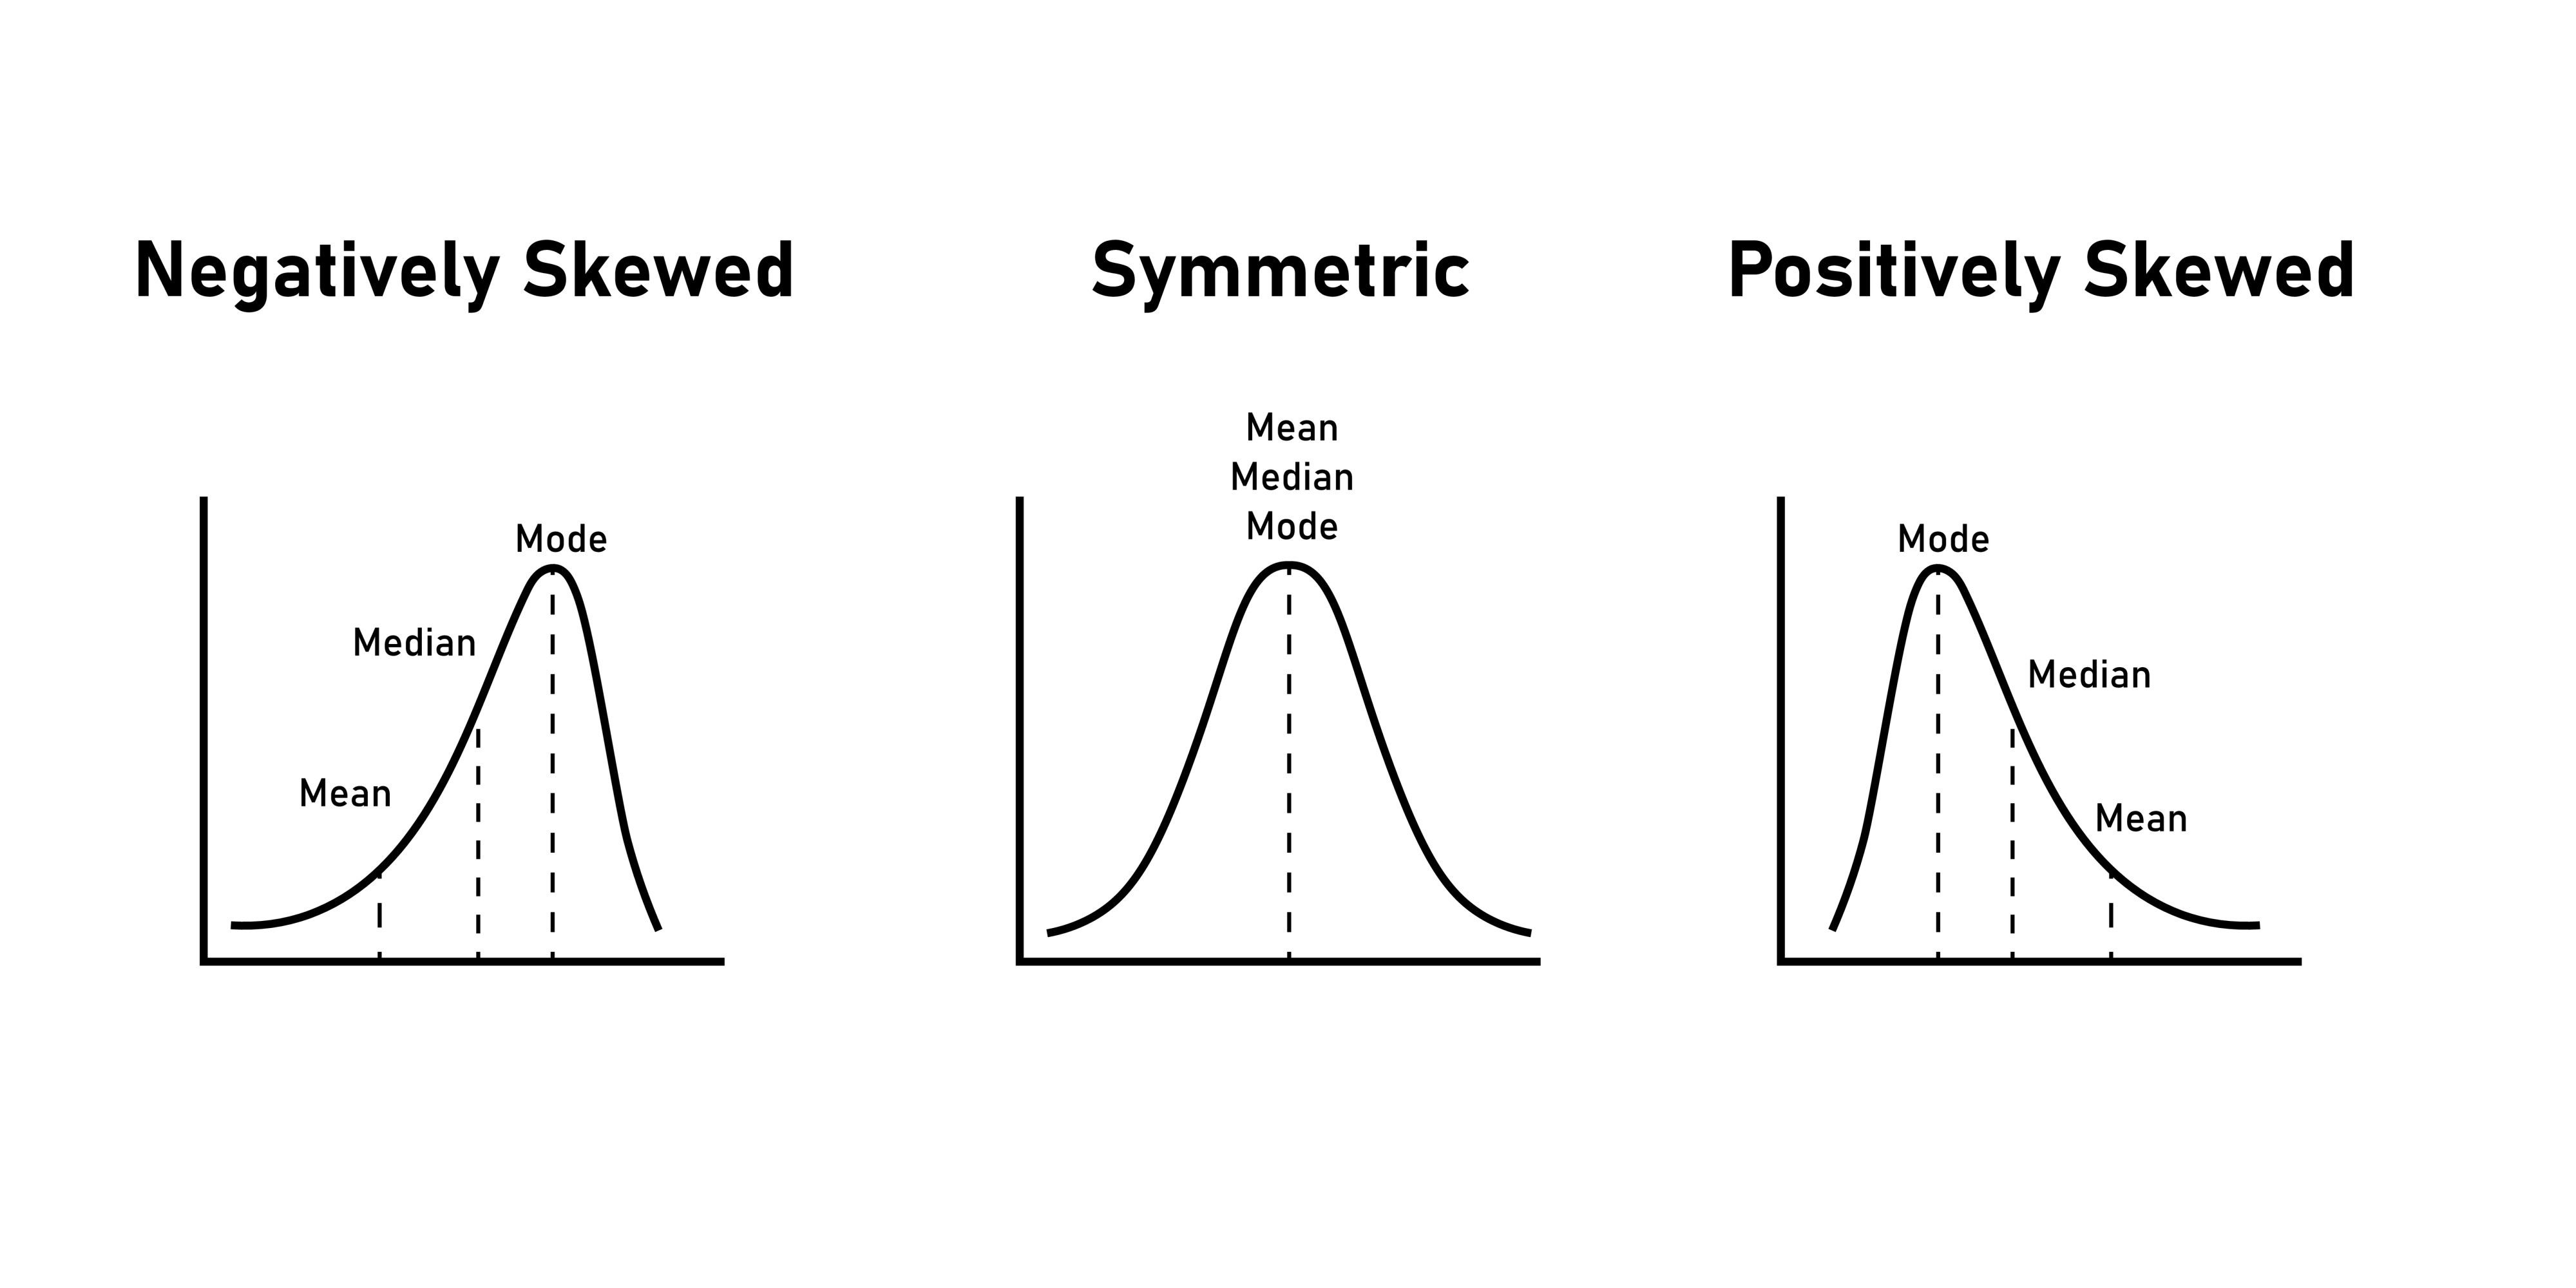
\includegraphics[width=0.7\textwidth]{imagenes/marco/skeweness.jpg}
	\caption{Comparison of negatively-skewed, symmetric and positively-skewed distributions \cite{pearson1895skewness}.}
	\label{fig:skewness}
\end{figure}

Taken together, these two diagnostics give an initial, coordinate-level read on how well the Gaussian approximation actually holds. Empirical evidence suggests that for many real-world datasets, both kurtosis and skewness values typically fall within the range $[-1,1]$ tails \cite{hair2019multivariate}, indicating distributions that are close to symmetric and free of excessively heavy.

\subsection{Per-Dimension Gaussianity: Moments and Formal Tests}
\label{sec:method:gaussianity:moments}
\phantomsection\label{sec:method:gaussianity:normaltest}

Building on the conceptual diagnostics above, we now formalize the per-dimension analysis into a concrete testing methodology. To verify Gaussianity at the level of individual feature coordinates, we apply three complementary indicators to every (class~$c$, dimension~$j$) pair.

\subsubsection{Shape moments.}
Following the normality diagnostics of Pearson~\cite{pearson1895skewness} and D'Agostino and Pearson~\cite{dagostino1971omnibus,dagostino1973tests}, we compute the sample skewness and excess kurtosis for each class~$c$ along each of the $d$ coordinates:
\begin{equation}
	\widehat{\mathrm{Skew}}_{c,j} \;=\; \frac{\frac{1}{n_c}\sum_{i}(x_{i,j}-\mu_{c,j})^3}{\hat\sigma_{c,j}^{3}},\qquad
	\widehat{\mathrm{Kurt}}_{c,j} \;=\; \frac{\frac{1}{n_c}\sum_{i}(x_{i,j}-\mu_{c,j})^4}{\hat\sigma_{c,j}^{4}} - 3,
	\label{eq:moments}
\end{equation}
where both quantities vanish exactly for a theoretical Gaussian distribution~\cite{pearson1895skewness,joyce2011kurtosis}.

\subsubsection{D'Agostino--Pearson omnibus test.}
The moments alone do not constitute a formal statistical test. We therefore apply the D'Agostino--Pearson omnibus test to every (class, dimension) pair~\cite{dagostino1971omnibus,dagostino1973tests}. The test combines the two shape statistics into a single composite statistic:
\begin{equation}
	K^2 \;=\; Z_1\!\left(\widehat{\mathrm{Skew}}\right)^2 + Z_2\!\left(\widehat{\mathrm{Kurt}}\right)^2 \;\sim\; \chi^2_2 \quad \text{under } H_0,
	\label{eq:normaltest}
\end{equation}
where $Z_1$ and $Z_2$ are normalised transformations of the skewness and kurtosis estimators respectively, and $H_0$ is the hypothesis that the marginal data are normally distributed. We reject $H_0$ at significance level $\alpha=0.05$.

\subsubsection{Relaxed criterion.}
Because the omnibus test is highly sensitive to larger sample sizes $n_c$ (where minor, non-critical departures from perfect normality still accumulate into significant $K^2$ values), we supplement it with a size-independent relaxed indicator. A dimension is classified as near-Gaussian if:
\begin{equation}
	|\mathrm{Skew}| < 1 \quad \text{and} \quad |\mathrm{Kurt}| < 1
\end{equation}
hold simultaneously. This relaxed criterion acts alongside the strict omnibus test to establish lower and upper bounds on the proportion of approximately Gaussian coordinates.

\subsection{The Henze--Zirkler Test}
\label{sec:method:gaussianity:hz_theory}

The diagnostics above operate one coordinate at a time, so they cannot pick up on dependencies between coordinates: a set of features can each look perfectly normal on their own while their joint distribution still departs from a proper multivariate Gaussian. The Henze--Zirkler (HZ) test~\cite{henze1990class} closes this gap: it is an omnibus test, applicable to a feature vector of any dimension $d$, that compares the empirical characteristic function of the data against the theoretical characteristic function of a multivariate normal distribution.

Given $n$ centred samples $\vec{z}_i = \vec{x}_i - \hat{\boldsymbol{\mu}}_c$ and a smoothing bandwidth $b > 0$, the test statistic is built from three terms evaluated using the squared Mahalanobis distances $d_M^2(\cdot,\cdot)$ induced by the class covariance $\boldsymbol{\Sigma}_c$:

\begin{equation}
	A = \frac{1}{n^2} \sum_{j=1}^{n} \sum_{k=1}^{n} e^{-\frac{b^2}{2}d_M^2(\vec{z}_j, \vec{z}_k)},
\end{equation}
\begin{equation}
	B = \frac{2}{n}(1+b^2)^{-d/2} \sum_{j=1}^{n} e^{-\frac{b^2}{2(1+b^2)}d_M^2(\vec{z}_j, \vec{0})},
\end{equation}
\begin{equation}
	C = (1+2b^2)^{-d/2}.
\end{equation}

Term $A$ measures the average pairwise kernel similarity of the observed samples; term $B$ quantifies how consistently the empirical density decays away from the class centroid compared to a Gaussian; and term $C$ is the asymptotic self-similarity constant of a true $d$-dimensional Gaussian. The final statistic is:
\begin{equation}
	T_{n,b} = n \cdot \left[ A - B + C \right].
\end{equation}

Under the null hypothesis of multivariate normality, $T_{n,b}$ converges to a fixed value close to $1$; departures above $1$ indicate that the data is more structured (tighter clusters or heavier tails) than a Gaussian. The bandwidth $b$ controls the resolution of the characteristic function comparison and is set optimally as a function of $n$ and $d$. The next two subsections apply this same statistic to two settings that differ only in dimensionality: first the univariate case ($d=1$), applied per coordinate as a stricter complement to the tests above, and then the full, high-dimensional multivariate case ($d=768$) that the classifier actually operates in.

\subsection{Univariate Henze-Zirkler Test per Dimension}
\label{sec:method:gaussianity:hz_univariate}

We bridge the per-dimension and per-class analyses by introducing a univariate HZ analysis applied independently to every (class~$c$, dimension~$j$) pair. This provides a stricter hypothesis-based criterion than the D'Agostino--Pearson test, while remaining more interpretable than the full-dimensional multivariate result presented next.

\paragraph{Bandwidth.}
For $d=1$, the standard HZ smoothing parameter reduces to:
\begin{equation}
	b^2 \;=\; \frac{1}{2}\left(\frac{4}{3}\right)^{2/5} n_c^{-2/5}.
	\label{eq:hz_bw_univariate}
\end{equation}

\paragraph{Efficient vectorised computation.}
To handle all $d$ dimensions simultaneously without forming prohibitive $n_c \times n_c$ distance matrices, the pairwise kernel term in $T_{\mathrm{HZ}}$ is expanded via its Taylor series around $b^2 x_j x_k = 0$:
\begin{equation}
	A_m \;=\; \frac{1}{n_c^2}\sum_{j,k} e^{-\frac{b^2}{2}(z_{j,m}-z_{k,m})^2}
	\;=\; \frac{1}{n_c^2}\sum_{\ell=0}^{L}
	\frac{b^{2\ell}}{\ell!}\,S_\ell^2\;+\;\mathcal{O}\!\left((b^2)^{L+1}\right),
	\label{eq:hz_taylor}
\end{equation}
where $S_\ell = \sum_j v_{j,m}\,z_{j,m}^\ell$, $v_{j,m} = \exp(-b^2 z_{j,m}^2 / 2)$, and $L=8$ terms are used to keep the approximation error below $10^{-6}$.

\paragraph{Expected value under $H_0$ and p-value.}
For a general $d$-dimensional problem, the asymptotic expected value of $T_{\mathrm{HZ}}$ under exact normality is:
\begin{equation}
	\mathbb{E}_{H_0}[T_{\mathrm{HZ}}] \;=\; 1 - (1 + 2b^2)^{-d/2},
	\label{eq:hz_expected_general}
\end{equation}
which is the reference used for the multivariate diagonal test of Section~\ref{sec:method:gaussianity:multivariate} ($d=768$): even a modest bandwidth causes $(1+2b^2)^{-d/2}\to 0$ for large $d$, driving $\mathbb{E}_{H_0}[T_{\mathrm{HZ}}]\to 1$.

For the univariate case ($d=1$) treated in this section, we instead use the exact finite-sample expectation, which includes higher-order correction terms that the large-$d$ asymptotic approximation of Equation~\eqref{eq:hz_expected_general} discards:
\begin{equation}
	\mathbb{E}_{H_0}[T_{\mathrm{HZ}}] \;=\; 1 - a^{-1/2}\left(1 + \frac{b^2}{a} + \frac{3b^4}{4a^2}\right), \qquad a = 1+2b^2,
	\label{eq:hz_expected_univariate}
\end{equation}
with $b^2$ given by the bandwidth of Equation~\eqref{eq:hz_bw_univariate}.

Under the null hypothesis $H_0$ of perfect univariate normality, we theoretically expect the empirical statistic $T_{\mathrm{HZ}}$ to be close to $0$. For the class sizes encountered here ($n_c \in [60,\,400]$), the adaptive bandwidth is small ($b^2 \approx 0.04$), which yields a baseline expectation of $\mathbb{E}_{H_0}[T_{\mathrm{HZ}}] \approx 0.04$. Consequently, any coordinate that is genuinely Gaussian will yield an empirical $T_{\mathrm{HZ}}$ value fluctuating tightly around this near-zero baseline, in contrast to the high-dimensional multivariate case where $T_{\mathrm{HZ}} \to 1$.

\subsection{Per-Class Gaussianity: Diagonal Henze--Zirkler Adaptation}
\label{sec:method:gaussianity:multivariate}

Having applied the HZ statistic one coordinate at a time, we now turn to its genuinely multivariate use: testing the joint, $d$-dimensional distribution of each class directly. Computing a standard full-covariance HZ test is mathematically intractable in high-dimensional spaces where the per-class sample size is smaller than the feature dimensionality ($n_c < d$). Under these conditions, the empirical covariance matrix becomes singular and non-invertible, preventing the calculation of standard Mahalanobis distances.

To circumvent this rank deficiency without resorting to destructive dimensionality reduction, we formulate a diagonal-covariance adaptation of the HZ test. The required Mahalanobis distances are computed analytically by inverting only the $d$ per-coordinate sample variances (effectively regularizing the space), with a numerical floor of $\varepsilon=10^{-10}$ applied to guard against inactive dimensions:
\begin{equation}
	\mathbb{E}[T_{\mathrm{HZ}}] \;=\; 1 - (1+2b^2)^{-d/2} \;\to\; 1 \quad \text{as } d \to \infty,
	\label{eq:hz_expected}
\end{equation}
meaning that values concentrated near $T_{\mathrm{HZ}} \approx 1$ serve as the Gaussian reference under the diagonal model.

Having established, at both the univariate and multivariate levels, how well class-conditional features actually satisfy the Gaussianity assumption, we now turn to how these Gaussians are positioned \emph{relative to one another} within the embedding space.

\section{Inter-Class Structural Separability Analysis}
\label{sec:method:separability}

To understand how the Bayesian decision surface scales and characterize the geometric crowding of the embedding space as new tasks are incorporated, we evaluate inter-class relationships using two complementary metrics: the probabilistic Bhattacharyya distance and the geometric Euclidean distance.

\subsection{Pairwise Bhattacharyya Distance}
\label{sec:method:separability:bhattacharyya}

The \emph{inter-class} pairwise Bhattacharyya distance measures how distinguishable any two class-conditional Gaussians are from one another.
The Bhattacharyya distance is symmetric and provides a direct connection to the Bayes error rate via the Bhattacharyya coefficient $\rho_{ij} = e^{-D_B(i,j)}$.
Under the diagonal-Gaussian parameterisation, the Bhattacharyya distance between classes $i$ and $j$ is defined as:
\begin{equation}
	D_B(i,j)
	= \frac{1}{8}(\boldsymbol{\mu}_i - \boldsymbol{\mu}_j)^{\top}
	\bar{\Sigma}^{-1}
	(\boldsymbol{\mu}_i - \boldsymbol{\mu}_j)
	+ \frac{1}{2}\ln\!\left(
	\frac{\det\bar{\Sigma}}{\sqrt{\det\Sigma_i\,\det\Sigma_j}}
	\right),
	\label{eq:interclass_bhattacharyya}
\end{equation}
where $\bar{\Sigma} = (\Sigma_i + \Sigma_j)/2$.
Because both $\Sigma_i$ and $\bar{\Sigma}$ are diagonal, all matrix operations reduce to element-wise arithmetic: determinants become products of the diagonal entries (or sums of logs), and the matrix inverse reduces to element-wise reciprocals.
A value of $D_B=0$ indicates complete distributional overlap; larger values correspond to greater separability and a lower Bhattacharyya coefficient $\rho = e^{-D_B}$.

\subsection{Pairwise Mean Euclidean Distance}
\label{sec:method:separability:euclidean}

While the Bhattacharyya distance jointly accounts for shifts in both first-order (means) and second-order (covariances) statistics, it can mask whether class texturing or raw prototype drift is the dominant factor in class confusion. Therefore, we isolate first-order geometric separation by calculating the plain pairwise Euclidean distance between the estimated class mean vectors $\boldsymbol{\mu}_i$ and $\boldsymbol{\mu}_j$:
\begin{equation}
	d_E(i,j) = \|\boldsymbol{\mu}_i - \boldsymbol{\mu}_j\|_2 = \sqrt{\sum_{k=1}^{d} (\mu_{i,k} - \mu_{j,k})^2},
	\label{eq:interclass_euclidean}
\end{equation}
where $d$ is the nominal dimensionality of the visual foundation embedding space.

\subsection{Stream Statistics and Trajectory Tracking}
\label{sec:method:separability:tracking}

As the total number of observed classes $k$ scales throughout the continual learning stream, we track three distinct statistics for both $D_B$ and $d_E$ across the expanding class-pair pool:
\begin{enumerate}
	\item[(a)] The \textbf{macro-averaged pairwise distance} ($\overline{D_B}$ and $\overline{d_E}$) flanked by a $[\mathrm{P}_{10},\mathrm{P}_{90}]$ percentile band to observe global drift.
	\item[(b)] The \textbf{minimum pairwise distance} ($\min D_B$ and $\min d_E$), which explicitly identifies the hardest, most confusable class pair in the system.
	\item[(c)] The \textbf{cumulative count of overlapping pairs} falling below critical proximity thresholds (e.g., $D_B \in \{10, 50, 100\}$ and $d_E \in \{0.3, 0.5, 0.7\}$) to capture the heavy-tailed growth of localized confusion sinks.
\end{enumerate}
Together, these metrics bridge empirical classification failure modes with the underlying statistical architecture of the learned representations.

The separability picture above already hints at why estimating each class's covariance matrix reliably matters so much: as classes crowd closer together, small errors in $\Sigma_c$ translate directly into decision-surface errors. We now look at why that estimation is difficult in the first place, and how it can be made reliable in the high-dimensional, small-sample regime this thesis operates in.

\section{Covariance Estimation in High-Dimensional Spaces}
\label{sec:gsc:covariance}

A fundamental challenge in multivariate statistical analysis and pattern recognition is the estimation of the covariance matrix $\boldsymbol{\Sigma} \in \mathbb{R}^{d \times d}$ from a finite set of $n$ observations. In classical low-dimensional regimes, where the sample size $n$ is much larger than the feature dimension $d$ ($n \gg d$), the empirical Sample Covariance Matrix (SCM) acts as a reliable, unbiased estimator. However, modern engineering applications—such as analyzing high-dimensional deep feature representations—frequently operate in the ``high-dimension, small-sample-size'' (HDSS) regime, where $d$ is of the order of hundreds or thousands, while $n$ remains strictly limited.

Under these conditions, classical multivariate analysis suffers severely from the \textit{curse of dimensionality}, leading to critical theoretical and numerical breakdowns in statistical modeling.

\subsection{The Curse of Dimensionality and Covariance Degeneracy}

When the dimensionality $d$ scales while the sample size $n$ remains fixed or grows at a slower rate, several geometric and algebraic anomalies emerge:

\begin{itemize}
	\item \textbf{Singularity and Rank Deficiency:} Structurally, the SCM is calculated as the sum of $n$ outer products of centered data vectors. Consequently, the maximum rank of the SCM is bounded by $\min(n-1, d)$. In the typical HDSS scenario where $n < d$, the SCM has at least $d - n + 1$ zero eigenvalues. The resulting matrix is singular (rank-deficient) and cannot be inverted.

	\item \textbf{Loss of Negative Log-Likelihood and Distance Metrics:} Many fundamental statistical classifiers and density estimators—such as Gaussian Discriminant Analysis (GDA) or Mahalanobis distance formulations—depend heavily on the precision matrix (the inverse covariance, $\boldsymbol{\Sigma}^{-1}$) and the log-determinant $\ln|\boldsymbol{\Sigma}|$. When the estimated covariance is singular, the log-determinant diverges to $-\infty$, and the precision matrix is undefined, rendering density estimation mathematically impossible.

	\item \textbf{Eigenvalue Distortion (Spreading Phenomenon):} Even in moderately high dimensions where $n \ge d$ and the SCM is technically invertible, the sample eigenvalues do not converge to their true counterparts. As proved in random matrix theory (e.g., the Marčenko-Pastur law \cite{MarPas67}), high-dimensional sample eigenvalues exhibit severe bias: the largest eigenvalues are systematically overestimated, while the smallest eigenvalues are underestimated. This artificial dispersion distorts the perceived geometric structure of the data.
\end{itemize}

\subsection{Theoretical Foundations of Regularization}

To overcome the numerical and structural instability of the empirical SCM in high dimensions, the theoretical framework must transition from pure maximum likelihood estimation toward \textit{regularization}. The conceptual objective is to trade a manageable amount of bias for a drastic reduction in estimator variance.

Conceptually, these regularized estimation strategies fall into two primary paradigms:

\begin{enumerate}
	\item \textbf{Spectral Regularization and Conditioning:} These approaches directly manipulate the empirical eigenspectrum. By placing a lower bound on near-zero eigenvalues or adding a perturbation matrix (e.g., diagonal loading), they artificially bound the condition number of the matrix. This guarantees strict positive definiteness ($\boldsymbol{\Sigma} \succ 0$), ensuring that the precision matrix remains numerically stable during inversion.

	\item \textbf{Structured Shrinkage:} Shrinkage theory, pioneered by Stein's loss formulations, constructs an estimator as a convex combination of the high-variance SCM and a low-variance structured ``target'' matrix (such as the identity matrix or a diagonal variance matrix). By shrinking the empirical estimator toward a well-behaved target, these methods systematically pull the distorted, spread-out eigenvalues back toward their true mean, minimizing the expected mean squared error.
\end{enumerate}

These two regularisation paradigms motivate the family of covariance estimators used throughout this thesis---diagonal, full, hybrid, shared, OAS, and Ledoit--Wolf---each trading a different amount of bias for a reduction in estimator variance. The eigenvalue anomalies described above are, at their root, a question of how variance is distributed across the $d$ coordinates of the feature space; we now turn to the spectral tools used to expose that distribution directly.

\section{Spectral Geometry and Dimensionality of the Feature Space}
\label{sec:gsc:spectral}

The validity of high-dimensional Gaussian modelling, and the practical behaviour of the covariance estimators just introduced, are both governed by the spectral structure of the embedding space: the way in which variance is distributed across the $d$ coordinates of the feature vector $\vec{x} \in \mathbb{R}^d$. We first develop Principal Component Analysis (PCA) as the analytical tool used to expose this structure, and then use it to define the effective dimensionality of the feature space and to design a controlled dimension-reduction probe.

\subsection{Principal Component Analysis}
\label{sec:marco:pca}

Principal Component Analysis (PCA) is a linear dimensionality-reduction technique that finds an orthonormal basis for the data by diagonalising the empirical covariance matrix~\cite{jolliffe2002principal}. Given a centred data matrix $\mathbf{X} \in \mathbb{R}^{N \times d}$ (zero-mean columns), the empirical covariance is

\begin{equation}
\mathbf{S} = \frac{1}{N-1}\mathbf{X}^{T}\mathbf{X}.
\end{equation}

Its eigendecomposition $\mathbf{S} = \mathbf{P}\boldsymbol{\Lambda}\mathbf{P}^{T}$ yields orthonormal eigenvectors $\mathbf{P} = [\mathbf{p}_1, \ldots, \mathbf{p}_d]$ sorted so that the corresponding eigenvalues satisfy $\lambda_1 \ge \lambda_2 \ge \cdots \ge \lambda_d \ge 0$. Each eigenvector $\mathbf{p}_i$ is a \emph{principal component} (PC), and $\lambda_i$ equals the variance of the data projected onto $\mathbf{p}_i$.

\paragraph{Dimensionality reduction.}
Retaining only the leading $k$ eigenvectors defines the projection matrix $\mathbf{P}_k = [\mathbf{p}_1, \ldots, \mathbf{p}_k] \in \mathbb{R}^{d \times k}$. A new observation $\vec{x} \in \mathbb{R}^d$ is mapped to a $k$-dimensional representation via

\begin{equation}
\tilde{\vec{x}} = \mathbf{P}_k^{T}(\vec{x} - \boldsymbol{\mu}),
\label{eq:pca_project}
\end{equation}

where $\boldsymbol{\mu}$ is the global mean estimated from the training corpus. The resulting coordinates $\tilde{\vec{x}}$ are decorrelated: $\operatorname{Cov}(\tilde{\vec{x}}) = \operatorname{diag}(\lambda_1, \ldots, \lambda_k)$. The fraction of total variance preserved by the projection is

\begin{equation}
R(k) = \frac{\sum_{i=1}^{k}\lambda_i}{\sum_{i=1}^{d}\lambda_i}.
\end{equation}

\paragraph{Optimality and geometric interpretation.}
Among all rank-$k$ linear projections, PCA minimises the mean-squared reconstruction error and maximises the variance of the projected data (Eckart--Young theorem~\cite{eckart1936approximation}). Geometrically, the projected subspace aligns with the axes of the data ellipsoid along which the observations spread most.

\paragraph{Application to high-dimensional embeddings.}
When the original dimension $d$ is large (e.g.\ $d=768$ for DINOv2 ViT-B/14) but the data occupy a low-dimensional subspace---as evidenced by rapid eigenvalue decay---reducing to $k \ll d$ dimensions before downstream classification offers two complementary benefits: (i) it concentrates the discriminative signal in fewer coordinates, potentially improving the accuracy of subsequent covariance estimators; and (ii) it reduces computational cost by a factor of $\mathcal{O}((d/k)^2)$ for quadratic (Mahalanobis) classifiers. The trade-off is that components beyond $k$ are discarded, which may remove residual discriminative information if the spectrum does not decay quickly enough.

\subsection{Spectral Decay and Effective Dimensionality}
\label{sec:gsc:spectral_decay}

The practical validity of high-dimensional Gaussian modeling is further supported by examining the spectral structure of the feature space through Principal Component Analysis. The covariance of the class-mean-centred embeddings can be decomposed as $\boldsymbol{\Sigma} = \mathbf{P}\boldsymbol{\Lambda}\mathbf{P}^T$, where the diagonal of $\boldsymbol{\Lambda}$ contains the eigenvalues $\lambda_1 \ge \lambda_2 \ge \dots \ge \lambda_d \ge 0$ and $\mathbf{P}$ holds the corresponding orthonormal eigenvectors.

\paragraph{Variance concentration.}
If the eigenvalue spectrum decays steeply---most variance is explained by the first $k \ll d$ components---then the effective dimensionality of the feature distribution is much lower than the nominal $d$. Concretely, the fraction of variance explained by the leading $k$ components is $\sum_{i=1}^{k}\lambda_i \,/\, \sum_{i=1}^{d}\lambda_i$.

\subsection{Global Spectral Analysis of the Foundation Embeddings}
\label{sec:method:spectral:analysis}

To characterize the global variance distribution of the foundation feature space independently of individual class-conditional labels, we compute the empirical eigenspectrum of the $\ell_2$-normalised embeddings pooled across the entirety of each benchmark's training split. The $d=768$ eigenvalues ($\lambda_1 \ge \lambda_2 \ge \dots \ge \lambda_d \ge 0$) of the pooled data covariance matrix are sorted in descending order to analyze individual percentage-of-variance contributions and the cumulative explained variance.

This diagnostic explicitly measures the \emph{effective intrinsic dimensionality} of the shared representation. A rapid, steep eigenvalue decay implies that the visual discriminative signal is concentrated within a tight, low-dimensional active subspace, pointing to high structural redundancy in the ambient space. Conversely, a slow, uniform decay indicates an isotropic distribution where discriminative information is scattered widely across the full ambient space. Furthermore, this global spectral profile establishes a strict theoretical upper bound on the effective rank available to the localized, per-class covariance estimators, as a class-specific model can only populate directional parameters already spanned by the pooled population spectrum.

\subsection{Downstream PCA Dimension-Reduction Probing}
\label{sec:method:spectral:pca_test}

While the spectral analysis of Section~\ref{sec:method:spectral:analysis} describes the native distribution of the features, it does not evaluate whether a low-dimensional concentration can be systematically exploited to alleviate the high-dimensional small-sample rank deficiency ($n_c < d$) highlighted in Section~\ref{sec:gsc:covariance}. To establish a diagnostic boundary on performance under forced compression, we introduce a downstream PCA dimension-reduction test.

Rather than fitting a localized, data-dependent Principal Component Analysis on each target stream---which would violate the strict class-incremental constraints by altering the projection matrix over time---we utilize a fixed, out-of-distribution linear projection matrix $\mathbf{P}_k \in \mathbb{R}^{d \times k}$. This projection matrix is pre-trained exclusively on the supervised distribution of the \emph{ImageNet-21k} corpus, acting as a general-purpose, dataset-agnostic structural probe.

For a chosen reduced target dimensionality $k \in \{64, 256\}$, the $\ell_2$-normalized foundation features $\mathbf{x} \in \mathbb{R}^d$ are projected into a compressed subspace via:
\begin{equation}
	\tilde{\mathbf{x}} = \mathbf{P}_k^{\top} (\mathbf{x} - \boldsymbol{\mu}_{\text{global}}),
	\label{eq:pca_projection}
\end{equation}
where $\boldsymbol{\mu}_{\text{global}}$ is the stationary global mean of the pre-training corpus. The class-conditional Gaussian classifiers (both Diagonal and Full covariance parameterisations) are subsequently initialized, trained, and evaluated entirely within this frozen, low-dimensional coordinate system.

The relative scaling of accuracy and estimator stability across these reduced dimensions serves as a multi-faceted probe into the underlying geometry:

The robustness of downstream CIL performance under forced compression ($k \ll d$) demonstrates an alignment between the current discriminative signal and the leading principal axes of the supervised out-of-distribution probe, confirming that trailing variances act primarily as non-essential noise. Conversely, a pronounced accuracy degradation alongside decreasing dimensionality reveals that fine-grained inter-class decision boundaries remain heavily reliant on the long tail of the spectrum, rendering the full ambient high-dimensional space mandatory for preserving the class representations.

Furthermore, the relative performance gap between the Full and Diagonal covariance models exposes the interaction between subspace compression and data scarcity. A narrowing of the gap at lower dimensionalities indicates that the regularizing effect of the projection successfully mitigates the small-sample rank deficiency of the SCM. In contrast, a wider divergence or a systemic drop in Full covariance precision points to a structural distortion of underlying class-conditional correlations induced by the linear transformation.

Having established the geometry of the feature space---its Gaussianity, its inter-class separability, and its spectral structure---this chapter's characterization of the feature space is complete. Chapter~\ref{ch:results} applies these tools to the empirical results of the proposed framework, beginning with the average accuracy and forgetting scores that quantify raw continual-learning performance, and, immediately after them, the confidence and calibration metrics used to judge how reliable those predictions actually are.
